\documentclass[main.tex]{subfiles}
\pagestyle{main} %%% pour compilation du sous document seul
%\setcounter{chapter}{1}

\begin{document}
\chapter{Optimisation de la reconstruction d'images scanners \label{chap:optim_grey}}
\mylettrine{M}{aintenant} que nous avons un modèle EDP qui reproduit bien les aspects constatés en clinique, interrogeons nous sur la manière de reconstruire une image en niveaux de gris (image scanner) à partir des résultats numériques \ie de l'évolution des densités~$N(t,x)$, $P(t,x)$ et~$S(t,x)$ (toutes comprises entre 0 et 1). Dans ce chapitre, on tentera d'optimiser les niveaux de gris~$\tau_N, \tau_P$ et~$\tau_S$ de l'interpolation EQREF \todo[noline]{eqref} afin de rapprocher au maximum la visualisation des résultats numériques de la visualisation des scanners médicaux.

\section{Présentation de l'approche}
Pour un patient donné, on considère~$n$ instants auxquels on possède des images scanners (aux temps~$t_i, i\in \{ 1,...,n \}$). Sur ces~$n$ images, on propose d'optimiser les coefficients (niveaux de gris) de l'interpolation~$\tau_N N + \tau_P P + \tau_S S$ où~$N, P$ et~$S$ sont les populations définies dans le modèle présenté précédemment. Sur l'ensemble de ces images, on fait correspondre le niveau de gris moyen des images numériques à celui des scanners, ce qui s'écrit~:
\begin{equation}
\label{eq:optim_grey_integ_aire}
\begin{aligned}
\frac{1}{\aire\big(Z_1(t_i)\big)}&\left( \tau_N\intperso{Z_1(t_i)}N(t_i,x) \dx + \tau_P\intperso{Z_1(t_i)}P(t_i,x) \dx + \tau_S\intperso{Z_1(t_i)} S(t_i,x) \dx \right) \\
&= \frac{1}{\aire\big(Z_2(t_i)\big)} \ \intperso{Z_2(t_i)} s(t_i,x,z_0) \dx \qquad i \in \{1,...,n\}
\end{aligned}
\end{equation}
où : \begin{myitemize}
\item $\aire(Z)$ est l'aire de la zone $Z$.
\item $Z_1(t_i)$ est la zone correspondant à la tumeur dans les simulations numériques au temps~$t_i$. Elle est définie par un seuillage sur~$S$.
\todo[noline]{specifier le seuillage ?}
\item $Z_2(t_i)$ est la zone tumorale sur le scanner réalisé au temps~$t_i$. Cette zone a été définie par contourage manuel à l'aide du logiciel OsiriX.
\item $z_0$ est la coupe que l'on choisit d'étudier dans les scanners. Cette coupe est approximativement la même au cours du temps de sorte à suivre l'évolution d'une même section du foie. 
\item $s(t_i,x,z_0)$ est la valeur du niveau de gris du pixel en position~$x$ sur la coupe~$z_0$ du scanner effectué au temps~$t_i$.
\end{myitemize}
En utilisant la discrétisation, aussi bien sur les simulations numériques que sur les scanners, on obtient :
\begin{equation}
\label{eq:optim_grey_eq_discr}
\begin{aligned}
\frac{1}{\mathcal{N}\big(Z_1(t_i)\big)}&\left( \tau_N\!\!\sum_{x\in Z_1(t_i)}\!\!N(t_i,x) + \tau_P\!\!\sum_{x\in Z_1(t_i)}\!\!P(t_i,x) + \tau_S\!\!\sum_{x\in Z_1(t_i)}\!\!S(t_i,x) \right) \\
&= \frac{1}{\mathcal{N}\big(Z_2(t_i)\big)} \sum_{x\in Z_2(t_i)}\!\! s(t_i,x,z_0) \qquad i \in \{1,...,n\}
\end{aligned}
\end{equation}
où~$\mathcal{N}(Z)$ désigne le nombre de pixels contenus dans la zone~$Z$. On a donc un système linéaire de 3 inconnues à~$n$ équations que l'on peut réécrire :
\begin{equation} \label{eq:Atau_egal_B}
A\tau=B,
\end{equation}
avec~$\tau= \trans(\tau_N,\tau_P,\tau_S)$, $A$ matrice de taille~$n\times 3$ et~$B$ vecteur colonne de taille~$n$.

Pour ne pas se limiter au cas~$n=3$ qui clôt le système, on le résout par la minimisation suivante :
\begin{equation}\label{eq:min_optim_grey}
\min_{\tau} J(\tau) \ \textrm{ avec } \ J(\tau)= \dfrac{\| A\tau - B \|^2_{\ell^2}}{\|B\|^2_{\ell^2}} + \mathcal{P}(\tau),
\end{equation}
où~$\mathcal{P}$ pénalise la fonction coût~$J$ lorsque l'une des composantes de~$\tau$ est en dehors de l'intervalle~$[0;255]$. 
%Dans la section qui suit, nous démarrerons avec une pénalisation en créneau
Une pénalisation en créneau sera considérée ici
\begin{equation}
\label{eq:penalisation_creneau}
\mathcal{P}(\tau) = 1e7 \times ( \tau \notin  [0;255]^3 ).
\end{equation}
%Dans la section d'après, la régularisée de Moreau-Yosida d'une parabole tronquée sera considérée comme pénalisation. Cette méthode de régularisation est décrite dans l'annexe REF page REF \todo[noline]{ref anex + page}. Dans cette annexe également, on examinera l'influence du choix de la fonction de pénalisation sur les optima fournit.
%permet d'assurer que les optima respectent les bornes~0 à~255 :


\section{Optimisation sur 3 paramètres}
%\DTLloaddb{optim3_0grey}{../data/cout_1/optim3.csv}
%\DTLloaddb[noheader]{optim3_0leg}{../data/cout_1/optim3_leg.csv}
%\DTLloaddb{optim3_0stat}{../data/cout_1/optim3_stat.csv}
%%\DTLloaddb[noheader]{optim3_0stat}{../data/cout_1/optim3_stat.csv}
%%\DTLsetheader{optim3_0stat}{Column1}{}
%\DTLsetheader{optim3_0leg}{Column1}{}
%\DTLsetheader{optim3_0leg}{Column2}{}
%\begin{sidewaystable}
%\footnotesize\smaller[0.5]
%%\scriptsize
%\centering
%\begin{tabular}{|c|c|c|c|c|}
%\hline
%%%\hhline{|>{\arrayrulecolor{white}}->{\arrayrulecolor{black}}|-|-|}
%\rowcolor{gray!70}
%& \multicolumn{4}{c|}{ \cellcolor{gray!70} \bfseries  Algorithme d'optimisation} \\
%\hhline{|>{\arrayrulecolor{gray!70}}->{\arrayrulecolor{black}}|-|-|-|-|}
%\rowcolor{gray!70}
%& \bfseries SLSQP
%& \bfseries GC 
%& \bfseries Neldear-Mead 
%& \bfseries BFGS \\
%\rowcolor{gray!70}
%\multirow{-3}{\firstcolwidth}{\scriptsize \bfseries \centering Scanners choisis pour l'optimisation}
%& $\tau_N, \qquad \tau_P, \qquad \tau_S$
%& $\tau_N, \qquad \tau_P, \qquad \tau_S$
%& $\tau_N, \qquad \tau_P, \qquad \tau_S$
%& $\tau_N, \qquad \tau_P, \qquad \tau_S$
%%%\\ \hline &&
%%%\\ \multicolumn{3}{|c|}{\rule{3cm}{1pt}}
%\DTLforeach*{optim3_0grey}{%
%\scan=scan,\NM=NM,\BFGS=BFGS,\col=SLSQP,\CG=CG,
%\errNM=errNM,\errBFGS=errBFGS,\errcol=errSLSQP,\errCG=errCG}{%
%\\
%\DTLifoddrow{\rowcolor{white}}{\rowcolor{gray!40}}%
%\scan & \begin{tabular}{c}
%\col \\ \errcol
%\end{tabular} & \begin{tabular}{c}
%\CG \\ \errCG
%\end{tabular} & \begin{tabular}{c}
%\NM \\ \errNM
%\end{tabular} & \begin{tabular}{c}
%\BFGS \\ \errBFGS
%\end{tabular} 
%}%
%\DTLforeach*{optim3_0stat}{%
%\NM=NM,\BFGS=BFGS,\col=SLSQP,\CG=CG}{%
%\\ \hline \hline %\DTLifoddrow{\rowcolor{white}}{\rowcolor{gray!40}}%
%Moyenne : & \col & \CG & \NM & \BFGS  }
%\\ \hline
%\end{tabular}
%\caption{\label{tab:optim3gris} Tableau récapitulatif des optimisations pour les 3 niveaux de gris}
%\end{sidewaystable}
%\DTLcleardb{optim3_0leg}
%\DTLcleardb{optim3_0stat}
%\DTLcleardb{optim3_0stat}


\DTLloaddb{optim3_0grey}{../data/cout_1/optim3.csv}
\DTLloaddb[noheader]{optim3_0leg}{../data/cout_1/optim3_leg.csv}
\DTLloaddb{optim3_0stat}{../data/cout_1/optim3_stat.csv}
%\DTLloaddb[noheader]{optim3_0stat}{../data/cout_1/optim3_stat.csv}
%\DTLsetheader{optim3_0stat}{Column1}{}
\DTLsetheader{optim3_0leg}{Column1}{}
\DTLsetheader{optim3_0leg}{Column2}{}
%\begin{sidewaystable}
%%\footnotesize\smaller[0.5]
%\scriptsize\smaller[2]
%\centering
%\begin{tabular}{|c|c|c|c|c|}
%\hline
%%%\hhline{|>{\arrayrulecolor{white}}->{\arrayrulecolor{black}}|-|-|}
%\rowcolor{gray!70}
%& \multicolumn{4}{c|}{ \cellcolor{gray!70} \bfseries  Algorithme d'optimisation} \\
%\hhline{|>{\arrayrulecolor{gray!70}}->{\arrayrulecolor{black}}|-|-|-|-|}
%\rowcolor{gray!70}
%& \bfseries SLSQP
%& \bfseries GC 
%& \bfseries Neldear-Mead 
%& \bfseries BFGS \\
%\rowcolor{gray!70}
%\multirow{-3}{\firstcolwidth}{\scriptsize \bfseries \centering Scanners choisis pour l'optimisation}
%& $\tau_N, \qquad \tau_P, \qquad \tau_S$
%& $\tau_N, \qquad \tau_P, \qquad \tau_S$
%& $\tau_N, \qquad \tau_P, \qquad \tau_S$
%& $\tau_N, \qquad \tau_P, \qquad \tau_S$
%%%\\ \hline &&
%%%\\ \multicolumn{3}{|c|}{\rule{3cm}{1pt}}
%\DTLforeach*{optim3_0grey}{%
%\scan=scan,\NM=NM,\BFGS=BFGS,\col=SLSQP,\CG=CG,
%\errNM=errNM,\errBFGS=errBFGS,\errcol=errSLSQP,\errCG=errCG}{%
%\\
%\DTLifoddrow{\rowcolor{white}}{\rowcolor{gray!40}}%
%\scan & \begin{tabular}{c}
%\col \\ \errcol
%\end{tabular} & \begin{tabular}{c}
%\CG \\ \errCG
%\end{tabular} & \begin{tabular}{c}
%\NM \\ \errNM
%\end{tabular} & \begin{tabular}{c}
%\BFGS \\ \errBFGS
%\end{tabular} 
%}%
%\DTLforeach*{optim3_0stat}{%
%\NM=NM,\BFGS=BFGS,\col=SLSQP,\CG=CG}{%
%\\ \hline \hline %\DTLifoddrow{\rowcolor{white}}{\rowcolor{gray!40}}%
%Moyenne : & \col & \CG & \NM & \BFGS  }
%\\ \hline
%\end{tabular}
%\caption{\label{tab:optim3gris} Tableau récapitulatif des optimisations pour les 3 niveaux de gris}
%\end{sidewaystable}

\begin{sidewaystable}
\footnotesize\smaller[0.5]
%\scriptsize
\centering
\begin{tabular}{|c|cc|cc|cc|cc|}
\hline
%%\hhline{|>{\arrayrulecolor{white}}->{\arrayrulecolor{black}}|-|-|}
\rowcolor{gray!70}
& \multicolumn{8}{c|}{ \cellcolor{gray!70} \bfseries  Algorithme d'optimisation} \\
\hhline{|>{\arrayrulecolor{gray!70}}->{\arrayrulecolor{black}}|--|--|--|--|}
\rowcolor{gray!70}
& \multicolumn{2}{|c|}{\cellcolor{gray!70} \bfseries SLSQP }
& \multicolumn{2}{c|}{ \cellcolor{gray!70} \bfseries GC }
& \multicolumn{2}{c|}{ \cellcolor{gray!70} \bfseries Neldear-Mead }
& \multicolumn{2}{c|}{\cellcolor{gray!70}  \bfseries BFGS } \\
\rowcolor{gray!70}
\multirow{-3}{\firstcolwidth}{\scriptsize \bfseries \centering Scanners choisis pour l'optimisation}
& $\tau_N, \qquad \tau_P, \qquad \tau_S $& Erreur
& $\tau_N, \qquad \tau_P, \qquad \tau_S $& Erreur
& $\tau_N, \qquad \tau_P, \qquad \tau_S $& Erreur
& $\tau_N, \qquad \tau_P, \qquad \tau_S $& Erreur
%%\\ \hline &&
%%\\ \multicolumn{3}{|c|}{\rule{3cm}{1pt}}
\DTLforeach*{optim3_0grey}{%
\scan=scan,\NM=NM,\BFGS=BFGS,\col=SLSQP,\CG=CG,
\errNM=errNM,\errBFGS=errBFGS,\errcol=errSLSQP,\errCG=errCG}{%
\\
\DTLifoddrow{\rowcolor{white}}{\rowcolor{gray!40}}%
\scan & 
\col &\errcol
&
\CG &\errCG
&
\NM & \errNM
&
\BFGS & \errBFGS
}%
\DTLforeach*{optim3_0stat}{%
\NM=NM,\BFGS=BFGS,\col=SLSQP,\CG=CG}{%
\\ \hline \hline %\DTLifoddrow{\rowcolor{white}}{\rowcolor{gray!40}}%
Moyenne : & \col && \CG && \NM && \BFGS &  }
\\ \hline
\end{tabular}
\caption{\label{tab:optim3gris} Tableau récapitulatif des optimisations pour les 3 niveaux de gris}
\end{sidewaystable}





\DTLcleardb{optim3_0leg}
\DTLcleardb{optim3_0stat}
\DTLcleardb{optim3_0stat}
La résolution de l'équation~\eqref{eq:min_optim_grey} fournit le~$\tau$ optimal. Il y a cependant plusieurs manières de calculer cet optimum. On peut  faire varier :
\begin{myitemize}
\item le nombre d'images considérées
\item les moments considérés
\item l'algorithme d'optimisation lui-même
%\item la fonction coût utilisée
\end{myitemize}

\todo[noline]{Presenter les algo}
Dans tous les cas, on ne considérera pas le premier scanner (numéro~0) car la condition initiale numérique EQREF \todo[noline]{EQREF} n'est pas prise de sorte à respecter la répartition des niveaux de gris du scanner. Evitons donc d'inclure dans l'optimisation une erreur de base qui serait incompressible. On regardera des situations avec seulement 2 images (problème sous-déterminé) ou 3 images (problème fermé) ou plus (problème sur-déterminé).

En ce qui concerne les algorithmes d'optimisations utilisés, nous en choisirons quatre~:
\begin{myitemize}
\item SLSQP (Sequential Least SQuares Programming)~: Méthodes des moindres carrés 
\item GC~: Gradient Conjugué
\item Neldear-Mead~: Algorithme basé sur une méthode du Simplex.
\item BFGS (Broyden, Fletcher, Goldfarb, and Shanno)~: Méthode quasi newtonnienne basée  également sur une approximation de la dérivée.
\todo[inline]{Ref : Piocher ref algo : \url{http://docs.scipy.org/doc/scipy-0.15.1/reference/generated/scipy.optimize.minimize.html} }
\end{myitemize}
Ces algorithmes seront initialisés avec les paramètres~$\tau_N, \tau_P$ et~$\tau_S$ de l'estimation visuelle du chapitre REF SECTION ET/OU PAGE \todo[noline]{ref section}. Lorsqu'il sont nécessaire, les gradients (voire les hessiennes) sont approximés par les algorithmes eux-mêmes. Outre un vecteur de paramètre initial et la fonction coût à optimiser~\eqref{eq:min_optim_grey}, aucune information supplémentaire n'est fournie à ces différents algorithmes.




\todo[noline]{Presenter numerotation des scans}
La Table~\ref{tab:optim3gris} synthétise une partie des résultats d'optimisation obtenus sur les différents tests qui ont été réalisés. 
On remarque que plus le nombre d'images considérées est grand, plus l'erreur à convergence a tendance à être grande. Ce comportement est attendu et ne pose pas de problème tant que l'erreur reste acceptable (de l'ordre de quelques pourcents). Augmenter le nombre d'images considérées s'avère utile pour rendre les optima moins sensibles aux perturbations éventuelles qu'il y a sur les données (bruit, marge d'erreur de segmentation manuelle, etc.).


On peut de plus remarquer que selon les images et les algorithmes choisis les résultats sont assez variables. Les moyennes des optima trouvés selon l'algorithme sont présentées sur la dernière ligne de la Table~\ref{tab:optim3gris}. Seul l'algorithme SLSQP se démarque des autres qui ont~:
\begin{myitemize}
\item une valeur moyenne de~$\tau_P$ supérieure à~$\tau_S$ alors qu'on s'attendrait plutôt à l'inverse...  Des images ont été reconstituées avec des valeurs de~$\tau_S$ aux alentours de 140 et 150. Il apparaît que la couleur du tissu sain n'est pas bonne~: il est beaucoup trop foncé. 
\item pour environ un tiers des combinaisons, une valeur de~$\tau_P$ proche de celle de~$\tau_S$, ce qui ne facilite pas du tout le contraste du tissu proliférant avec le tissu sain.
\end{myitemize}
L'algorithme Neldear-Mead semble le moins bon algorithme, au vu notamment des résultats fournis pour les combinaisons~[1,9,11], [2,3,4,5] et~[3,5,7] qui font apparaître une valeur de $\tau_N$ de~255~! Non seulement elle est grande, mais en plus elle atteint le bord autorisé. Notez que si l'on retire ces 3 valeurs de la moyenne présentée sur la dernière ligne du tableau, alors celle-ci s'approche des moyennes des algorithmes GC et BFGS. 


Pour expliquer l'erreur commise sur~$\tau_S$, on pourrait penser à une large variabilité permise sur ce paramètre due à la présence très minoritaire de tissu sain dans la tumeur. Ainsi~$\tau_S$ serait très peu influent dans le calcul de l'erreur~\eqref{eq:min_optim_grey}. Cependant après avoir examiné de plus près les valeurs des intégrales de l'équation~\eqref{eq:optim_grey_integ_aire} (\ie les coefficients de la matrice~$A$), il y a toujours au moins 10\% de cellules saines. La plupart du temps, elles sont réparties sur le pourtour de la tumeur, dans la zone de transition sur laquelle il y a un mélange de tissu sain et de tissu tumoral. Ceci écarte donc l'hypothèse avancée. On pourrait alors avancer des variations dans les données (bruit dans les images, erreur sur le contourage, variation du temps d'acquisition du scanner qui impacte les niveaux de gris, ... ) pour justifier cela, mais les impacts sont difficiles à mesurer. 
Il n'en reste pas moins que le niveau de gris~$\tau_S$ est mal estimé. 
Pour palier à cela, nous allons le fixer dans la section suivante.


%%%%%  ---- SECTION  OPTIM SUR 2 NVX DE GRIS ----- %%%%%
\section{Optimisation sur 2 paramètres, $\tau_S$ fixé \label{sec:optim_2_param}}
Pour essayer de palier aux problèmes rencontrés dans la section précédente, nous allons fixer~$\tau_S$ à une valeur de 197 (sur l'échelle des niveaux de gris de~0 à~255). Cette valeur a été fixée en réalisant un contourage d'une zone de tissu sain dans OsiriX (\cf  Figure~\ref{fig:contourage_sain}). La moyenne de ce contourage est de~134.5 HU. Le niveau de gris étant échelonné linéairement entre~-135 et~215, on peut ainsi faire correspondre cette quantité en HU à un niveau de gris compris entre~0 et~255 (\cf Figure~\ref{fig:schema_correspondance_gris}). Ainsi, selon l'échelle considérée ici, 134.5~HU est  équivalent à un gris de 77\% soit un gris de niveau~197.

\begin{figure}
\centering
\begin{figure}
\centering
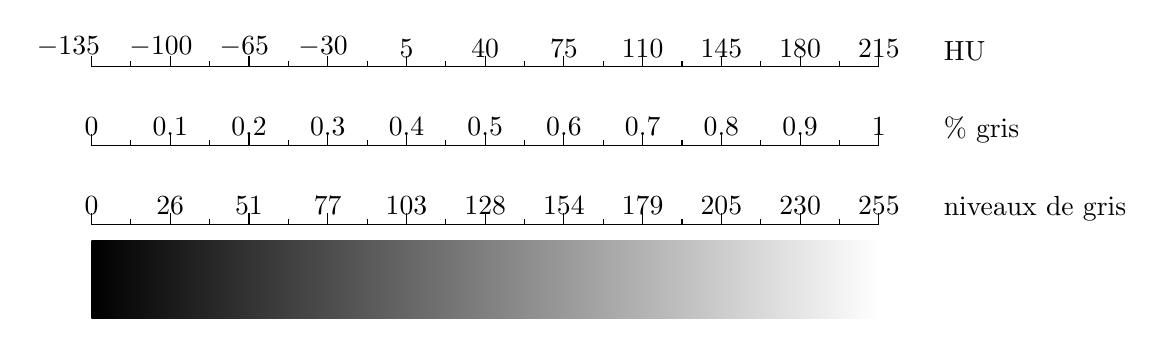
\begin{tikzpicture}
  \shade[left color=black, right color=white] (0,0) rectangle (10,1);   
  \draw (0,1.2) -- (10,1.2) ;
  \draw (0,2.2) -- (10,2.2) ;
  \draw (0,3.2) -- (10,3.2) ;
  \foreach \x/\xtexta/\xtextb/\xtextc in {0/0/0/-135\ \ \ \ \  ,
  1/0.1/26/-100\ \ , %%%pour forcer des espaces
  2/0.2/51/-65\ , 
  3/0.3/77/-30\ , 
  4/0.4/103/5, 
  5/0.5/128/40, 
  6/0.6/154/75, 
  7/0.7/179/110, 
  8/0.8/205/145, 
  9/0.9/230/180, 
  10/1/255/215}{
    \draw[shift={(\x,1.2)}] (0pt,4pt) -- (0pt,0pt) node[above] {$\xtextb$};    
    \draw[shift={(\x,2.2)}] (0pt,4pt) -- (0pt,0pt) node[above] {$\xtexta$};
    \draw[shift={(\x,3.2)}] (0pt,4pt) -- (0pt,0pt) node[above] {$\xtextc$};
    }
  \foreach \x in {0,1,2,3,4,5,6,7,8,9}{
  	\draw[shift={(\x+0.5,1.2)}] (0pt,2pt) -- (0pt,0pt) ; 
  	\draw[shift={(\x+0.5,2.2)}] (0pt,2pt) -- (0pt,0pt) ;
  	\draw[shift={(\x+0.5,3.2)}] (0pt,2pt) -- (0pt,0pt) ;
  	}
  	\draw (10.7,3.4) node[right] {HU};   
  	\draw (10.7,2.4) node[right] { \% gris}; 
  	\draw (10.7,1.4) node[right] {niveaux de gris};     
\end{tikzpicture}
\caption{\label{fig:schema_correspondance_gris} Correspondance des niveaux de gris }
\end{figure}
\todo[noline]{Titre figure \ref{fig:schema_correspondance_gris} à revoir ...}
\caption{\label{fig:schema_correspondance_gris} Correspondance des niveaux de gris }
\end{figure}
\todo[noline]{Titre figure \ref{fig:schema_correspondance_gris} à revoir ...}


\begin{figure}
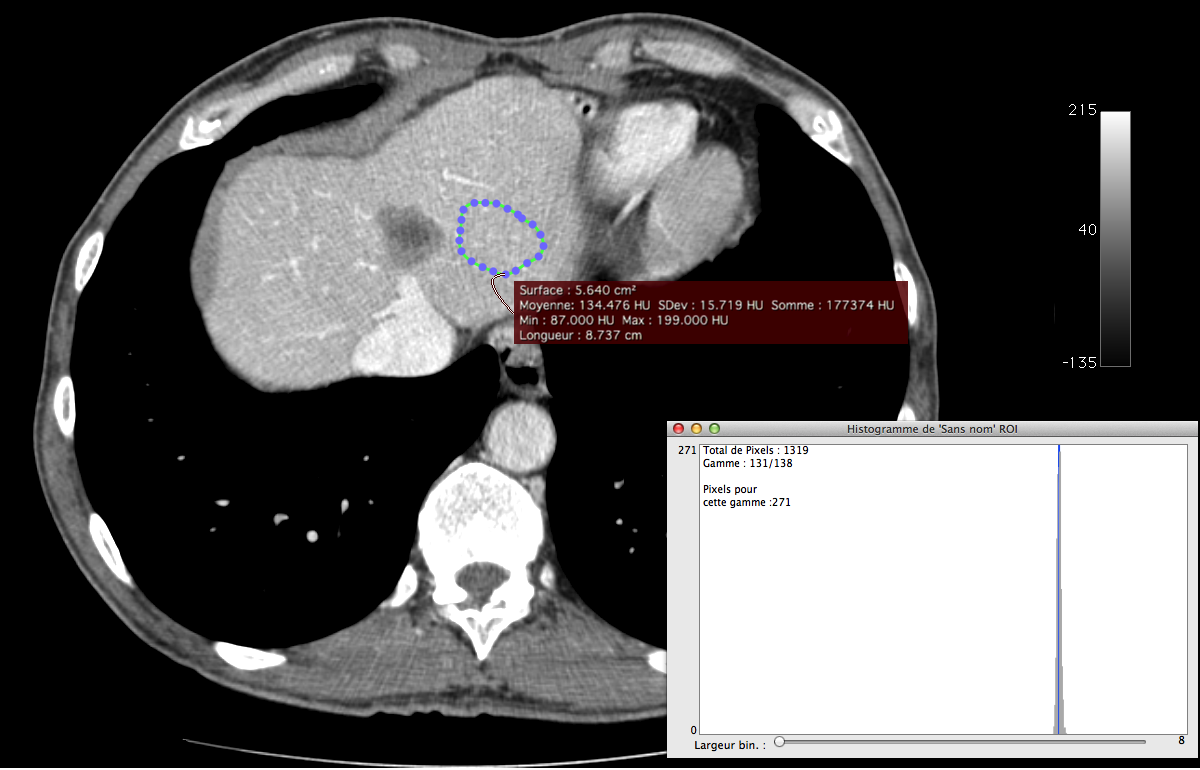
\includegraphics[width=\textwidth]{OsiriX_gris_sain_rognee.png}
\caption{\label{fig:contourage_sain}Contourage d'une zone saine réalisé à l'aide du logiciel OsiriX -- Moyenne de la valeur des pixels dans ce périmètre : 134.5 HU (avec une échelle HU de \mbox{-135 à 215}).}
\end{figure}

%%%%%% Cout1
%\DTLloaddb{optim2_1grey}{../data/cout_1/optim2.csv}
%\DTLloaddb[noheader]{optim2_1leg}{../data/cout_1/optim2_leg.csv}
%\DTLloaddb{optim2_1stat}{../data/cout_1/optim2_stat.csv}
\DTLloaddb{optim2_1grey}{../data/cout_1_good/optim2.csv}
\DTLloaddb[noheader]{optim2_1leg}{../data/cout_1_good/optim2_leg.csv}
\DTLloaddb{optim2_1stat}{../data/cout_1_good/optim2_stat.csv}


\DTLsetheader{optim2_1leg}{Column1}{}
\DTLsetheader{optim2_1leg}{Column2}{}
\begin{table}[h]
%\vspace{-35mm}
\centering
\footnotesize\smaller[0.5]
%\hspace{\retraittableau} %%% Le tableau depasse sur les marges !
\begin{tabular}{|c|c|c|c|c|}
\hline
%%\hhline{|>{\arrayrulecolor{white}}->{\arrayrulecolor{black}}|-|-|}
\rowcolor{gray!70}
& \multicolumn{4}{c|}{ \cellcolor{gray!70} \bfseries  Algorithme d'optimisation} \\
\hhline{|>{\arrayrulecolor{gray!70}}->{\arrayrulecolor{black}}|-|-|-|-|}
\rowcolor{gray!70}
& \bfseries SLSQP
& \bfseries GC 
& \bfseries Neldear-Mead 
& \bfseries BFGS \\
\rowcolor{gray!70}
\multirow{-3}{\firstcolwidth}{\scriptsize \bfseries \centering Scanners choisis pour l'optimisation}
& $\tau_N, \qquad \tau_P$
& $\tau_N, \qquad \tau_P$
& $\tau_N, \qquad \tau_P$
& $\tau_N, \qquad \tau_P$
\DTLforeach*{optim2_1grey}{%
\scan=scan,\NM=NM,\BFGS=BFGS,\col=SLSQP,\CG=CG,
\errNM=errNM,\errBFGS=errBFGS,\errcol=errSLSQP,\errCG=errCG}{%
\\
\DTLifoddrow{\rowcolor{white}}{\rowcolor{gray!40}}%
\scan & \begin{tabular}{c}
\col \\ Err : \errcol
\end{tabular} & \begin{tabular}{c}
\CG \\ Err : \errCG
\end{tabular} & \begin{tabular}{c}
\NM \\ Err : \errNM
\end{tabular} & \begin{tabular}{c}
\BFGS \\ Err : \errBFGS
\end{tabular} 
}%
\DTLforeach*{optim2_1stat}{%
\NM=NM,\BFGS=BFGS,\col=SLSQP,\CG=CG}{%
\\ \hline \hline %\DTLifoddrow{\rowcolor{white}}{\rowcolor{gray!40}}%
Moyenne : & \col & \CG & \NM & \BFGS  }
\\ \hline
\end{tabular}
%\centering
%\begin{tabular}{cc}
%\DTLdisplaydb{optim2_leg}
%\end{tabular}
\caption{\label{tab:optim2gris}Tableau récapitulatif des optimisations réalisées sur 2 niveaux de gris, $\tau_S$ fixé à 197, avec un créneau comme pénalisation de l'intervalle -- cas favorables }
%%\vspace{-4cm}
\end{table}
\DTLcleardb{optim2_1leg}
\DTLcleardb{optim2_1stat}
\DTLcleardb{optim2_1grey}


%%%%%%%%%%%%%%%%%%%%%%%%%%%

\DTLloaddb{optim2_1bgrey}{../data/cout_1_bad/optim2.csv}

\begin{table}[h]
%\vspace{-35mm}
\footnotesize\smaller[0.5]
\centering
%%\hspace{\retraittableau} %%% Le tableau depasse sur les marges !
\begin{tabular}{|c|c|c|c|c|}
\hline
%%\hhline{|>{\arrayrulecolor{white}}->{\arrayrulecolor{black}}|-|-|}
\rowcolor{gray!70}
& \multicolumn{4}{c|}{ \cellcolor{gray!70} \bfseries  Algorithme d'optimisation} \\
\hhline{|>{\arrayrulecolor{gray!70}}->{\arrayrulecolor{black}}|-|-|-|-|}
\rowcolor{gray!70}
& \bfseries SLSQP
& \bfseries GC 
& \bfseries Neldear-Mead 
& \bfseries BFGS \\
\rowcolor{gray!70}
\multirow{-3}{\firstcolwidth}{\scriptsize \bfseries \centering Scanners choisis pour l'optimisation}
& $\tau_N, \qquad \tau_P$
& $\tau_N, \qquad \tau_P$
& $\tau_N, \qquad \tau_P$
& $\tau_N, \qquad \tau_P$
\DTLforeach*{optim2_1bgrey}{%
\scan=scan,\NM=NM,\BFGS=BFGS,\col=SLSQP,\CG=CG,
\errNM=errNM,\errBFGS=errBFGS,\errcol=errSLSQP,\errCG=errCG}{%
\\
\DTLifoddrow{\rowcolor{white}}{\rowcolor{gray!40}}%
\scan & \begin{tabular}{c}
\col \\ Err : \errcol
\end{tabular} & \begin{tabular}{c}
\CG \\  Err : \errCG
\end{tabular} & \begin{tabular}{c}
\NM \\ Err : \errNM
\end{tabular} & \begin{tabular}{c}
\BFGS \\ Err : \errBFGS
\end{tabular} 
}%
\\ \hline
\end{tabular}
\caption{\label{tab:optim2gris_bad}Tableau récapitulatif des optimisations réalisées sur 2 niveaux de gris, $\tau_S$ fixé à 197, avec un créneau comme pénalisation de l'intervalle -- cas défavorables.}
%%\vspace{-4cm}
\end{table}
\DTLcleardb{optim2_1bgrey}

%%%%%%% Tableau conditionnement
\DTLloaddb{optim2_1bcond}{../data/cout_1_bad/optim2_cond.csv}
\DTLloaddb{optim3_1bcond}{../data/cout_1_bad/optim3_cond.csv}
\DTLloaddb{optim2_1gcond}{../data/cout_1_good/optim2_cond.csv}
\DTLloaddb{optim3_1gcond}{../data/cout_1_good/optim3_cond.csv}


%\DTLforeach*{optim3_1bcond}{%
%\scan=scan, \condi=ratio_s}{%
%%%\DTLifinlist{element}{list}{true part}{false part}
%\DTLifinlist{\condi}{ -}{\DTLremovecurrentrow}{
%\dtlreplaceentryincurrentrow{aaa}{ \dtlcolumnindex{optim3_1bcond}{ratio_s}  }
%}
%}%

\begin{table}[h]
\centering
%\vspace{-35mm}
\footnotesize
%\begin{tabular}{|c|m{3cm}|}
%\hline
%%%\hhline{|>{\arrayrulecolor{white}}->{\arrayrulecolor{black}}|-|-|}
%\rowcolor{gray!70} & \\
%\rowcolor{gray!70} &  \\
%\rowcolor{gray!70}
%\multirow{-3}{\firstcolwidth}{\scriptsize \bfseries \centering Scanners choisis pour l'optimisation}
%& \multirow{-3}{\firstcolwidth}{\scriptsize \bfseries \centering Conditionnement matrice 3x3}
%\DTLforeach*{optim3_1bcond}{%
%\scan=scan, \condi=ratio_s}{%
%\\
%\DTLifoddrow{\rowcolor{white}}{\rowcolor{gray!40}}%
%\scan & \condi
%}%
%\\ \hline \hline
%\DTLforeach*{optim3_1gcond}{%
%\scan=scan, \condi=ratio_s}{%
%\DTLiffirstrow{}{\\ \DTLifoddrow{\rowcolor{white}}{\rowcolor{gray!40}} }
%\scan & \condi
%}%
%\\ \hline
%\end{tabular}\hspace{4mm}
%\begin{tabular}{|c|m{3cm}|}
%\hline
%%%\hhline{|>{\arrayrulecolor{white}}->{\arrayrulecolor{black}}|-|-|}
%\rowcolor{gray!70} & \\
%\rowcolor{gray!70} &  \\
%\rowcolor{gray!70}
%\multirow{-3}{\firstcolwidth}{\scriptsize \bfseries \centering Scanners choisis pour l'optimisation}
%& \multirow{-3}{\firstcolwidth}{\scriptsize \bfseries \centering Conditionnement matrice 2x2}
%\DTLforeach*{optim2_1bcond}{%
%\scan=scan, \condi=ratio_s}{%
%\\
%\DTLifoddrow{\rowcolor{white}}{\rowcolor{gray!40}}%
%\scan & \condi
%}%
%\\ \hline \hline
%\DTLforeach*{optim2_1gcond}{%
%\scan=scan, \condi=ratio_s}{%
%\DTLiffirstrow{}{\\ \DTLifoddrow{\rowcolor{white}}{\rowcolor{gray!40}} }
%\scan & \condi
%}%
%\\ \hline
%\end{tabular}
%%%\vspace{-4cm}

\rowcolors{2}{gray!40}{white}
\begin{tabular}{|c|m{3cm}|}
\hline
%%\hhline{|>{\arrayrulecolor{white}}->{\arrayrulecolor{black}}|-|-|}
\rowcolor{gray!70} & \\
\rowcolor{gray!70} &  \\
\rowcolor{gray!70}
\multirow{-3}{\firstcolwidth}{\scriptsize \bfseries \centering Scanners choisis pour l'optimisation}
& \multirow{-3}{\firstcolwidth}{\scriptsize \bfseries \centering Conditionnement matrice 3x3} \\
$[2,3,4]$ & 1.5e+07  \\
$[2,3,5]$ & 2.8e+05 \\
$[2,5,7]$ & 3.1e+06 \\
$[1,7,11]$ & 1.8e+03 \\
$[1,9,11]$ & 1.6e+07 \\
$[3,5,7]$ & 4.7e+06 \\ \hline \hline
$[1,2,3]$ & 6.7e+02 \\
$[1,3,5]$ & 1.5e+02 \\
$[1,2,5]$ & 6.9e+01 \\
$[1,2,9]$ & 2.2e+01 \\ \hline
\end{tabular}\hspace{4mm}
\begin{tabular}{|c|m{3cm}|}
\hline
%%\hhline{|>{\arrayrulecolor{white}}->{\arrayrulecolor{black}}|-|-|}
\rowcolor{gray!70} & \\
\rowcolor{gray!70} &  \\
\rowcolor{gray!70}
\multirow{-3}{\firstcolwidth}{\scriptsize \bfseries \centering Scanners choisis pour l'optimisation}
& \multirow{-3}{\firstcolwidth}{\scriptsize \bfseries \centering Conditionnement matrice 2x2} \\
$[2,3]$ & 1.2e+05 \\ \hline \hline
$[1,2]$ & 1.6e+01 \\
$[1,3]$ & 1.8e+01 \\ \hline
\end{tabular}
\caption{\label{tab:condi2} Conditionnement (rapport de la plus grande valeur propre sur la plus petite).}
\end{table}
\DTLcleardb{optim2_1bcond}
\DTLcleardb{optim3_1bcond}
\DTLcleardb{optim2_1gcond}
\DTLcleardb{optim3_1gcond}





Ainsi nous résolvons toujours~\eqref{eq:Atau_egal_B}, mais ici avec
\begin{equation}
\label{eq:corresp_A_integ}
\begin{aligned}
A_{k,...}.\tau & = \frac{1}{\mathcal{N}\big(Z_1(t_i)\big)}\left( \tau_N\!\!\sum_{x\in Z_1(t_i)}\!\!N(t_i,x) + \tau_P\!\!\sum_{x\in Z_1(t_i)}\!\!P(t_i,x) \right), \\
B_k &= \frac{1}{\mathcal{N}\big(Z_2(t_i)\big)} \sum_{x\in Z_2(t_i)}\!\! s(t_i,x,z_0) - \bar{\tau_S}\!\!\sum_{x\in Z_1(t_i)}\!\!S(t_i,x) \qquad i \in \{1,...,n\},
\end{aligned}
\end{equation}
où~$A_{k,...}$ désigne la k-ième ligne de la matrice~$A$ et où~$\bar{\tau_S}$ est fixé à~197.


Les premiers essais ont été réalisés avec la même fonction coût \eqref{eq:min_optim_grey} et avec la même pénalisation~\eqref{eq:penalisation_creneau} que pour l'optimisation sur 3 paramètres. 
L'ensemble des résultats d'optimisation de~$\tau_N$ et de~$\tau_P$ avec~$\tau_S$ fixé à~197  %%et (( avec une parabole tronquée régularisée comme pénalisation ))\todo{penalisation} 
est fourni dans les Tables~\ref{tab:optim2gris} et~\ref{tab:optim2gris_bad}. 


La table~\ref{tab:optim2gris} présente les cas correctement convergés. Ici les niveaux de gris moyens fournis sont conformes aux attentes dans le sens où l'on a~$\tau_N$<$\tau_P$<$\tau_S$.  Une nouvelle fois, l'algorithme basé sur la méthode des moindres carrés se démarque des 3 autres qui fournissent des optima très similaires.


Cependant dans certaines configurations, présentées dans la Table~\ref{tab:optim2gris_bad}, les algorithmes tendent vers un jeu de paramètres optimal qui s'approche du bord 0 ou du bord 255, voire qui est négatif (\ie non convergence de l'algorithme d'optimisation). 
Même en écartant les configurations qui tendent vers le bord~0, il reste encore quelques combinaisons qui paraissent très pathologiques avec~$\tau_N$>>$\tau_S$ ce qui est aberrant. 
Notons que l'algorithme basé sur la méthode des moindres carrés semble moins touché par ce problème. 
Ces erreurs pourraient être dues notamment au fait que la pénalisation choisie \eqref{eq:penalisation_creneau} présente une discontinuité. Les algorithmes de descente fonctionnant sur une approximation du gradient peuvent ainsi être perturbés par cette discontinuité  aux abords des bornes autorisées. Dans l'annexe~\ref{chap:anx_penalisation} page~\pageref{chap:anx_penalisation} est détaillée l'enquête menée sur les fonctions de pénalisation. Des pénalisations plus régulières ont été testées (parabole tronquée et parabole tronquée régularisée) mais n'améliorent que très peu le résultat final. Ceci nous amène à penser que ce n'est donc pas la régularité de la pénalisation qui est à mettre en cause mais les données elles-mêmes. Certaines combinaisons d'images fourniraient donc de mauvais résultats. 




Pour une combinaison de 2 ou 3 images, on s'attend à ce que l'optimum soit la solution exacte du système linéaire, et ce indépendamment de l'algorithme choisi. Dans la mesure où ce n'est pas le cas, nous devons nous interroger sur le conditionnement des systèmes que l'on résout. S'ils ne 
sont pas bien conditionnés, alors une petite perturbation des données entraîne un très grand écart sur la solution du système. Bien que nous ne résolvions pas directement le système, mais que nous effectuions une minimisation, ces problèmes de sensibilité aux données n'ont aucune raison de ne pas se reporter. La Table~\ref{tab:condi2} présente les conditionnements (rapport de la plus grande valeur propre sur la plus petite) associés aux différentes combinaisons d'images que nous avons examinées. Pour les cas ayant bien convergé (partie inférieure des tableaux), le conditionnement reste raisonnable (excepté peut-être pour le cas~[1,2,3]). Maintenant, si on examine les cas ayant mal convergé, on constate des conditionnements très élevés (dans la partie supérieure des tableaux, les conditionnements dépassent~$10^3$). Le conditionnement semble donc expliquer la plupart des configurations non convergentes avec~2 ou~3 images. Pour les configurations où l'on considère un plus grand nombres d'images, si un sous-ensemble d'images fournit une configuration instable, alors il y a de fortes chances que l'image (ou les 2 images) supplémentaire(s) ne parvienne(nt) pas à contrebalancer cette instabilité. On pourra donner comme  exemple la configuration~[2,5,7] pour laquelle l'ajout de l'image n°1 ne fournit pas d'amélioration (\cf. résultats de la configuration~[1,2,5,7]) ou bien la configuration~[1,3,5,7] qui n'améliore pas la configuration~[3,5,7] ou encore la configuration~[1,3,7,11] qui n'améliore pas non plus la configuration~[1,7,11].


Pour les configurations contenant l'image n°11, on peut aussi avancer que le modèle EDP n'est pas proche de la réalité en terme de volume tumoral (\cf Figure~REFF\todo{ref}). Bien qu'ici les niveaux de gris soit moyennés, il y a certainement des erreurs qui se reportent sur nos systèmes.

\section{Conclusion}
L'algorithme basé sur la méthode des moindres carrés semble plus robuste que les autres méthodes examinées. Malgré tout, il peut également fournir des résultats biaisés dans le cas de système mal conditionnés. Il est donc important d'examiner le conditionnement -- ou du moins le conditionnement des sous-systèmes carrés -- pour donner de la crédibilité (ou non) aux optima fournis.

Dans les cas bien conditionnés,  les optima fournis sont relativement proches les uns des autres même en faisant varier la méthode d'optimisation ou bien les images considérées comme en atteste la Table~\ref{tab:optim2gris}. Dans la suite de ce manuscrit, on fixera alors les niveaux de gris~$\tau_N=25$, $\tau_P=143$ et~$\tau_S=197$.


\end{document}